\section{하위 조이스틱 JCR}
\label{sec:vla}

\begin{figure*}[t]
\centering
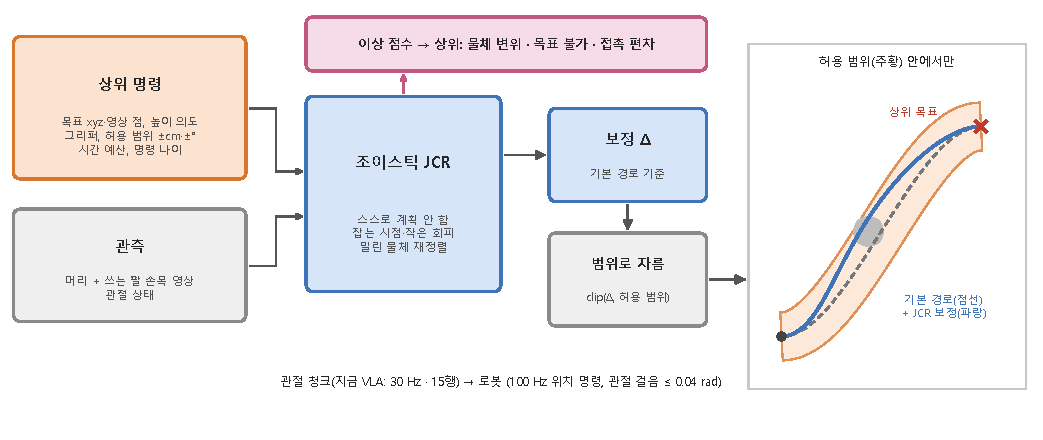
\includegraphics[width=\linewidth]{figures/f3_vla.pdf}
\caption{\textbf{조이스틱 JCR.} 상위 명령(목표·의도·그리퍼·허용 범위·명령 나이)과 관측을 받아, 명령이 만든 기본 경로에 대한 보정을 TCP 변위 청크로 내고 허용 범위로 자른다. 오른쪽: 기본 경로(점선)와 JCR 보정(파랑)은 허용 범위(주황) 밖으로 나가지 않는다. 이상 신호는 상위를 일찍 다시 부르는 근거가 된다.}
\label{fig:vla}
\end{figure*}

\paragraph{역할.} JCR(Joystick-Conditioned Reflex, 조이스틱 반사 정책)는 세 가지만 맡는다. (i) 조이스틱 따라가기, 곧 상위 명령 기준의 미세 조종, (ii) 잡기·놓기 시점, (iii) 접촉 여부 판단이다. 계획·단계 선택·목표 결정은 하지 않고 언어 명령도 받지 않는다(\cref{fig:vla}). 설계·데이터·학습·평가는 모두 상위가 명령을 준다는 전제 위에 있다. 시뮬 참값 명령은 상한을 재는 데만 쓴다.

\paragraph{입력.} 머리·쓰는 팔 손목 영상과 고정된 짧은 문장(단계 문장 없음), 그리고 조건 네 가지다. 조이스틱 $j$는 상위 목표 $-$ 손끝이며, 몸통 고정 좌표계의 연속 3D 값으로 양자화나 사각지대가 없다. 허용 범위는 목표 구 반경, 경로 관 반경, 허용 그리퍼 방향이다. 명령 나이는 명령이 나온 뒤 지난 시간이다. 고유 감각은 관절, 그리퍼 폭·전류(effort), 인과 후방 차분 속도, 현재 명령 관절이다. 단계 문장을 빼는 이유는 그리퍼 시점이 접촉이 아니라 문장에 붙기 때문이다(\cref{sec:evidence}).

\paragraph{출력과 권한.} 팔 행동은 현재 명령 TCP 기준의 변위 청크다(20\,Hz, 10행 = 0.5\,s, 0.2\,s마다 새 청크). 손끝 방향과 IK(중력 처짐 보정, 관절 한 걸음 0.04\,rad 이하)는 코드가 맡는다. 그리퍼는 행마다 \{유지, 닫기, 열기\} 사건을 내고, 접촉 확률 두 개(패드--대상, 예상 밖 접촉)를 낸다. 이상 신호는 별도 이진 머리(예상 밖 접촉, 대상 이동, 떨어짐, 명령 불일치, 복구 불가)와 멈춤 출력이며, 문턱은 보류 세트에서 등각(conformal) 방식으로 오탐률 5\,\%에 맞춘다~\cite{faildetect2025}. 실행되는 움직임은
\begin{equation}
  a_t = a^{\text{nom}}_t + \mathrm{clip}\bigl(\Delta_t,\ \mathcal{E}(c)\bigr),
\end{equation}
이며 $a^{\text{nom}}$은 명령 $c$가 만든 기본 경로, $\mathcal{E}(c)$는 명령이 허용한 범위다. 자름과 허용 그리퍼 방향은 코드가 강제하므로 JCR가 틀려도 상위 명령에서 범위 이상 벗어나지 않는다. 바탕 모델은 Qwen3-VL-4B~\cite{qwen3vl2025} LoRA 백본과 흐름 정합 행동 전문가이며, 전문가에서 백본으로 가는 기울기는 막는다~\cite{kinsulate2025}.

\paragraph{정답: 허용 범위에 투영한 시뮬 참값.} 참값 목표 $c^\ast$는 특권 물체 자세로 계산한 실제 잡기·놓기 자세를 허용 범위(목표 구 $\cup$ 경로 관)에 투영한 점이다. 명령이 조금 틀렸으면 JCR는 범위 안에서 실제 물체 쪽으로 고치고(미세 조종), 명령이 전혀 다른 곳을 가리키면 $c^\ast$는 범위 경계, 곧 조이스틱 쪽이 된다(따라가기). 한 정의로 두 역할이 나오고, 권한은 늘 상위에 있다. 범위를 벗어난 명령도 경계까지 따르고 명령 불일치 신호를 올린다. 참값 청크는 최소 저크 모양(속도 $\le$ 0.08\,m/s, 가속 $\le$ 0.32\,m/s$^2$)이고, 닫기 참값은 특권 쥐기 술어가 처음 참이 되는 틱, 열기 참값은 놓기 자세 1\,cm 안, 접촉 참값은 시뮬 접촉 센서 힘 $>$ 0.1\,N이다. 스냅샷마다 가짜 조이스틱 네 개(먼 구간 0.5--8\,cm, 근접 0.3--2\,cm)에 참값 청크를 짝지은 반사실 분기를 넣고, 분기는 시뮬 재생으로 실행 가능성을 확인한다(계획 대 실측 TCP 변위 차 중앙 $\le$ 3\,mm).

\paragraph{자기 롤아웃 재라벨.} 참값은 상태만의 함수이므로 JCR 자신이 돈 롤아웃의 방문 상태에서 다시 계산해 붙인다. 라벨을 내는 쪽은 학습된 정책이 아니라 특권 상태 함수이므로 교사 정책이 아니다. 라운드마다 기초 데이터와 모든 재라벨 데이터를 합쳐 처음부터 다시 학습하며, 교정 데이터만으로 이어 학습하지 않는다. 이 반복이 폐루프에서 생기는 상태 분포 이동을 없애는 수단이다.

\paragraph{실패와 외란.} 실패·외란은 버리지 않고 일부러 만든다. 물체 밀기, 미끄러짐, 장애물, 잡기 직전 대상 흔들기, 그리고 상위 명령의 점 오차·의도 오류·지연·도중 교체·미리 내기다. 규칙은 문헌을 따른다.
\begin{itemize}
  \item 실패 편에서 실행된 행동은 행동 복제 라벨로 쓰지 않는다. 방문 상태만 남기고 행동은 시뮬 참값 교정으로 바꾼다~\cite{crdagger2025,rac2025}. 이득 토큰 조건화~\cite{recap2025}는 쓰지 않는다.
  \item 정상 흐름은 절반 이상으로 두고, 교란 구간 안에서는 `범위로 복귀' 대 `과제 진행'을 1:1--1:2로 맞춘다. 교란 뒤 3\,s 안에 복구하지 못한 긴 꼬리는 자른다~\cite{rac2025}.
  \item 교란 크기는 JCR 자신의 오차 분포와 성공률에 맞춰 단계적으로 키운다~\cite{laskey2017dart}.
  \item 복구 불가 상태(탁자 밖으로 떨어짐, 넘어져 닿을 수 없음, 관절 한계)는 참값 교정기로 이어 돌린 반사실 롤아웃으로 판정하고, 정답은 억지 보정이 아니라 `이상 신호 + 멈춤'이다. 다시 계획하는 것은 상위다.
  \item 관측으로 알아볼 수 없는 교정(숨은 미끄러짐 등)은 행동 정답 대신 이상 신호로 보낸다.
\end{itemize}
틱마다 단계, 명령원, 외란 종류·시점, 편 결과를 남겨 같은 기록을 상위의 진행 평가·실패 감지 학습에도 쓸 수 있게 한다.

\paragraph{명령원.} 편의 30\,\%는 시뮬 참값 명령, 70\,\%는 상위 흉내 명령으로 만든다. 상위 흉내 명령은 본 35B 오프라인 평가에서 잰 경험 분포(점 오차, 동작 오류율, 호출 지연)를 머리 영상 픽셀 $\rightarrow$ 깊이 $\rightarrow$ xyz 경로로 주입하고, 갱신 간격 2--6\,s, 도중 교체 10\,\%, 도착 전 미리 받기 30\,\%를 더한다.

\paragraph{학습 4단계.} 정답은 모두 시뮬 참값(특권 정보로 계산)이다.
\begin{enumerate}
  \item \textbf{단독:} 참값·상위 흉내 명령 위에서 교란 장면의 참값 보정을 배우고, 자기 롤아웃 재라벨을 되풀이한다. 데이터 관문은 보정이 범위 안인지, 관절 걸음 $\le$ 0.04\,rad인지, 분기 실행 검증, 접촉 라벨 프레임 검수다.
  \item \textbf{상위 오차 흉내:} 주입 비중과 크기를 본 35B 최적 체크포인트의 오차·지연 분포로 맞춘다.
  \item \textbf{실제 상위와:} 실제 상위를 붙여 돈 기록에서 참값 보정으로 다시 학습해, 연결 지점의 분포 차이를 없앤다.
  \item \textbf{번갈아:} 상위와 서로의 실제 출력 위에서 번갈아 맞춘다(\cref{sec:mesh}).
\end{enumerate}
단독 성능표(참값 명령·상위 흉내 명령에서의 성공률, 교란 복구율, 접촉·이상 신호 정밀도·재현율, 그리퍼 시점 오차)는 1단계 뒤에 만들고, H-J 비교의 기준선이 된다(\cref{sec:eval}).
